\section{Data Preprocessing}
\subsection{Missing Value Analysis}
Initial analysis revealed missing values in three key variables:
\begin{itemize}
    \item Teacher Quality
    \item Parental Education Level
    \item Distance from Home
\end{itemize}

These missing values were handled using K-Nearest Neighbors (KNN) imputation, which preserves the relationships between variables while providing realistic estimates for the missing data.

\section{Continuous Variables Analysis}
\subsection{Correlation Analysis}
\begin{figure}[H]
    \centering
    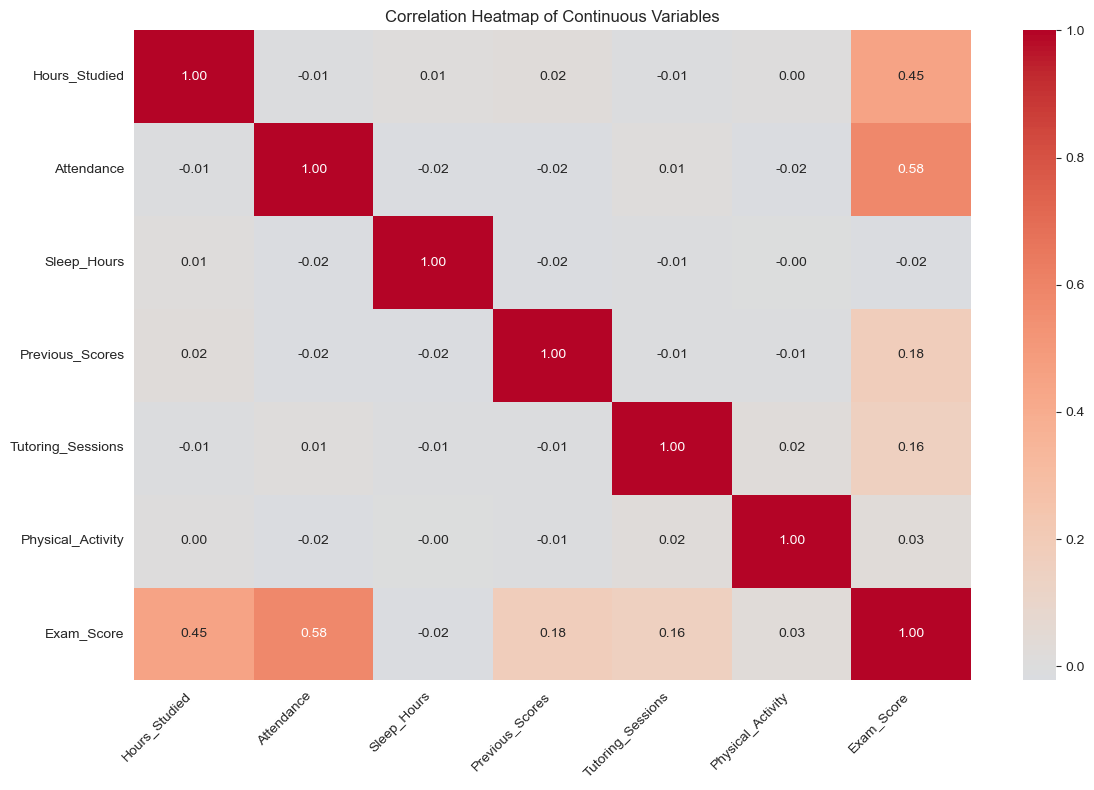
\includegraphics[width=0.8\textwidth]{images/correlation_heatmap.png}
    \caption{Correlation Heatmap of Continuous Variables}
\end{figure}

The correlation analysis revealed several significant relationships:
\begin{itemize}
    \item Strong positive correlation between Previous Scores and Exam Scores
    \item Moderate positive correlation between Study Hours and Exam Scores
    \item Weak to moderate correlations among other continuous variables
\end{itemize}

\subsection{Multicollinearity Assessment}
Variance Inflation Factor (VIF) analysis was performed to detect multicollinearity:
\begin{figure}[H]
    \centering
    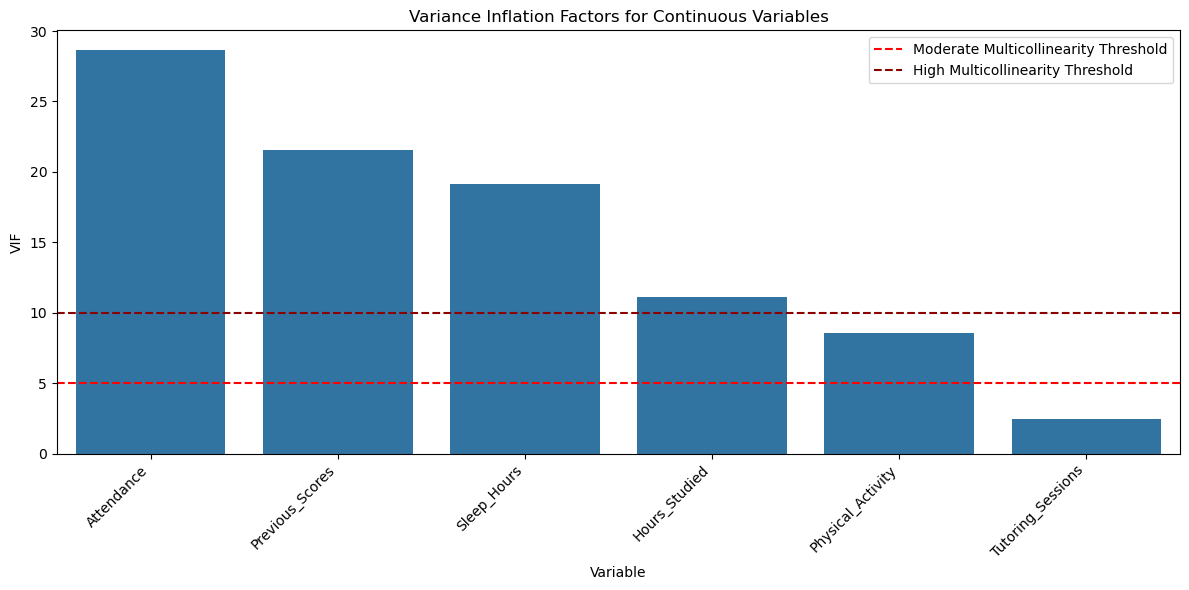
\includegraphics[width=0.8\textwidth]{images/vif_scores.png}
    \caption{Variance Inflation Factors for Continuous Variables}
\end{figure}

\section{Categorical Variables Analysis}
\subsection{Distribution Analysis}
\begin{figure}[H]
    \centering
    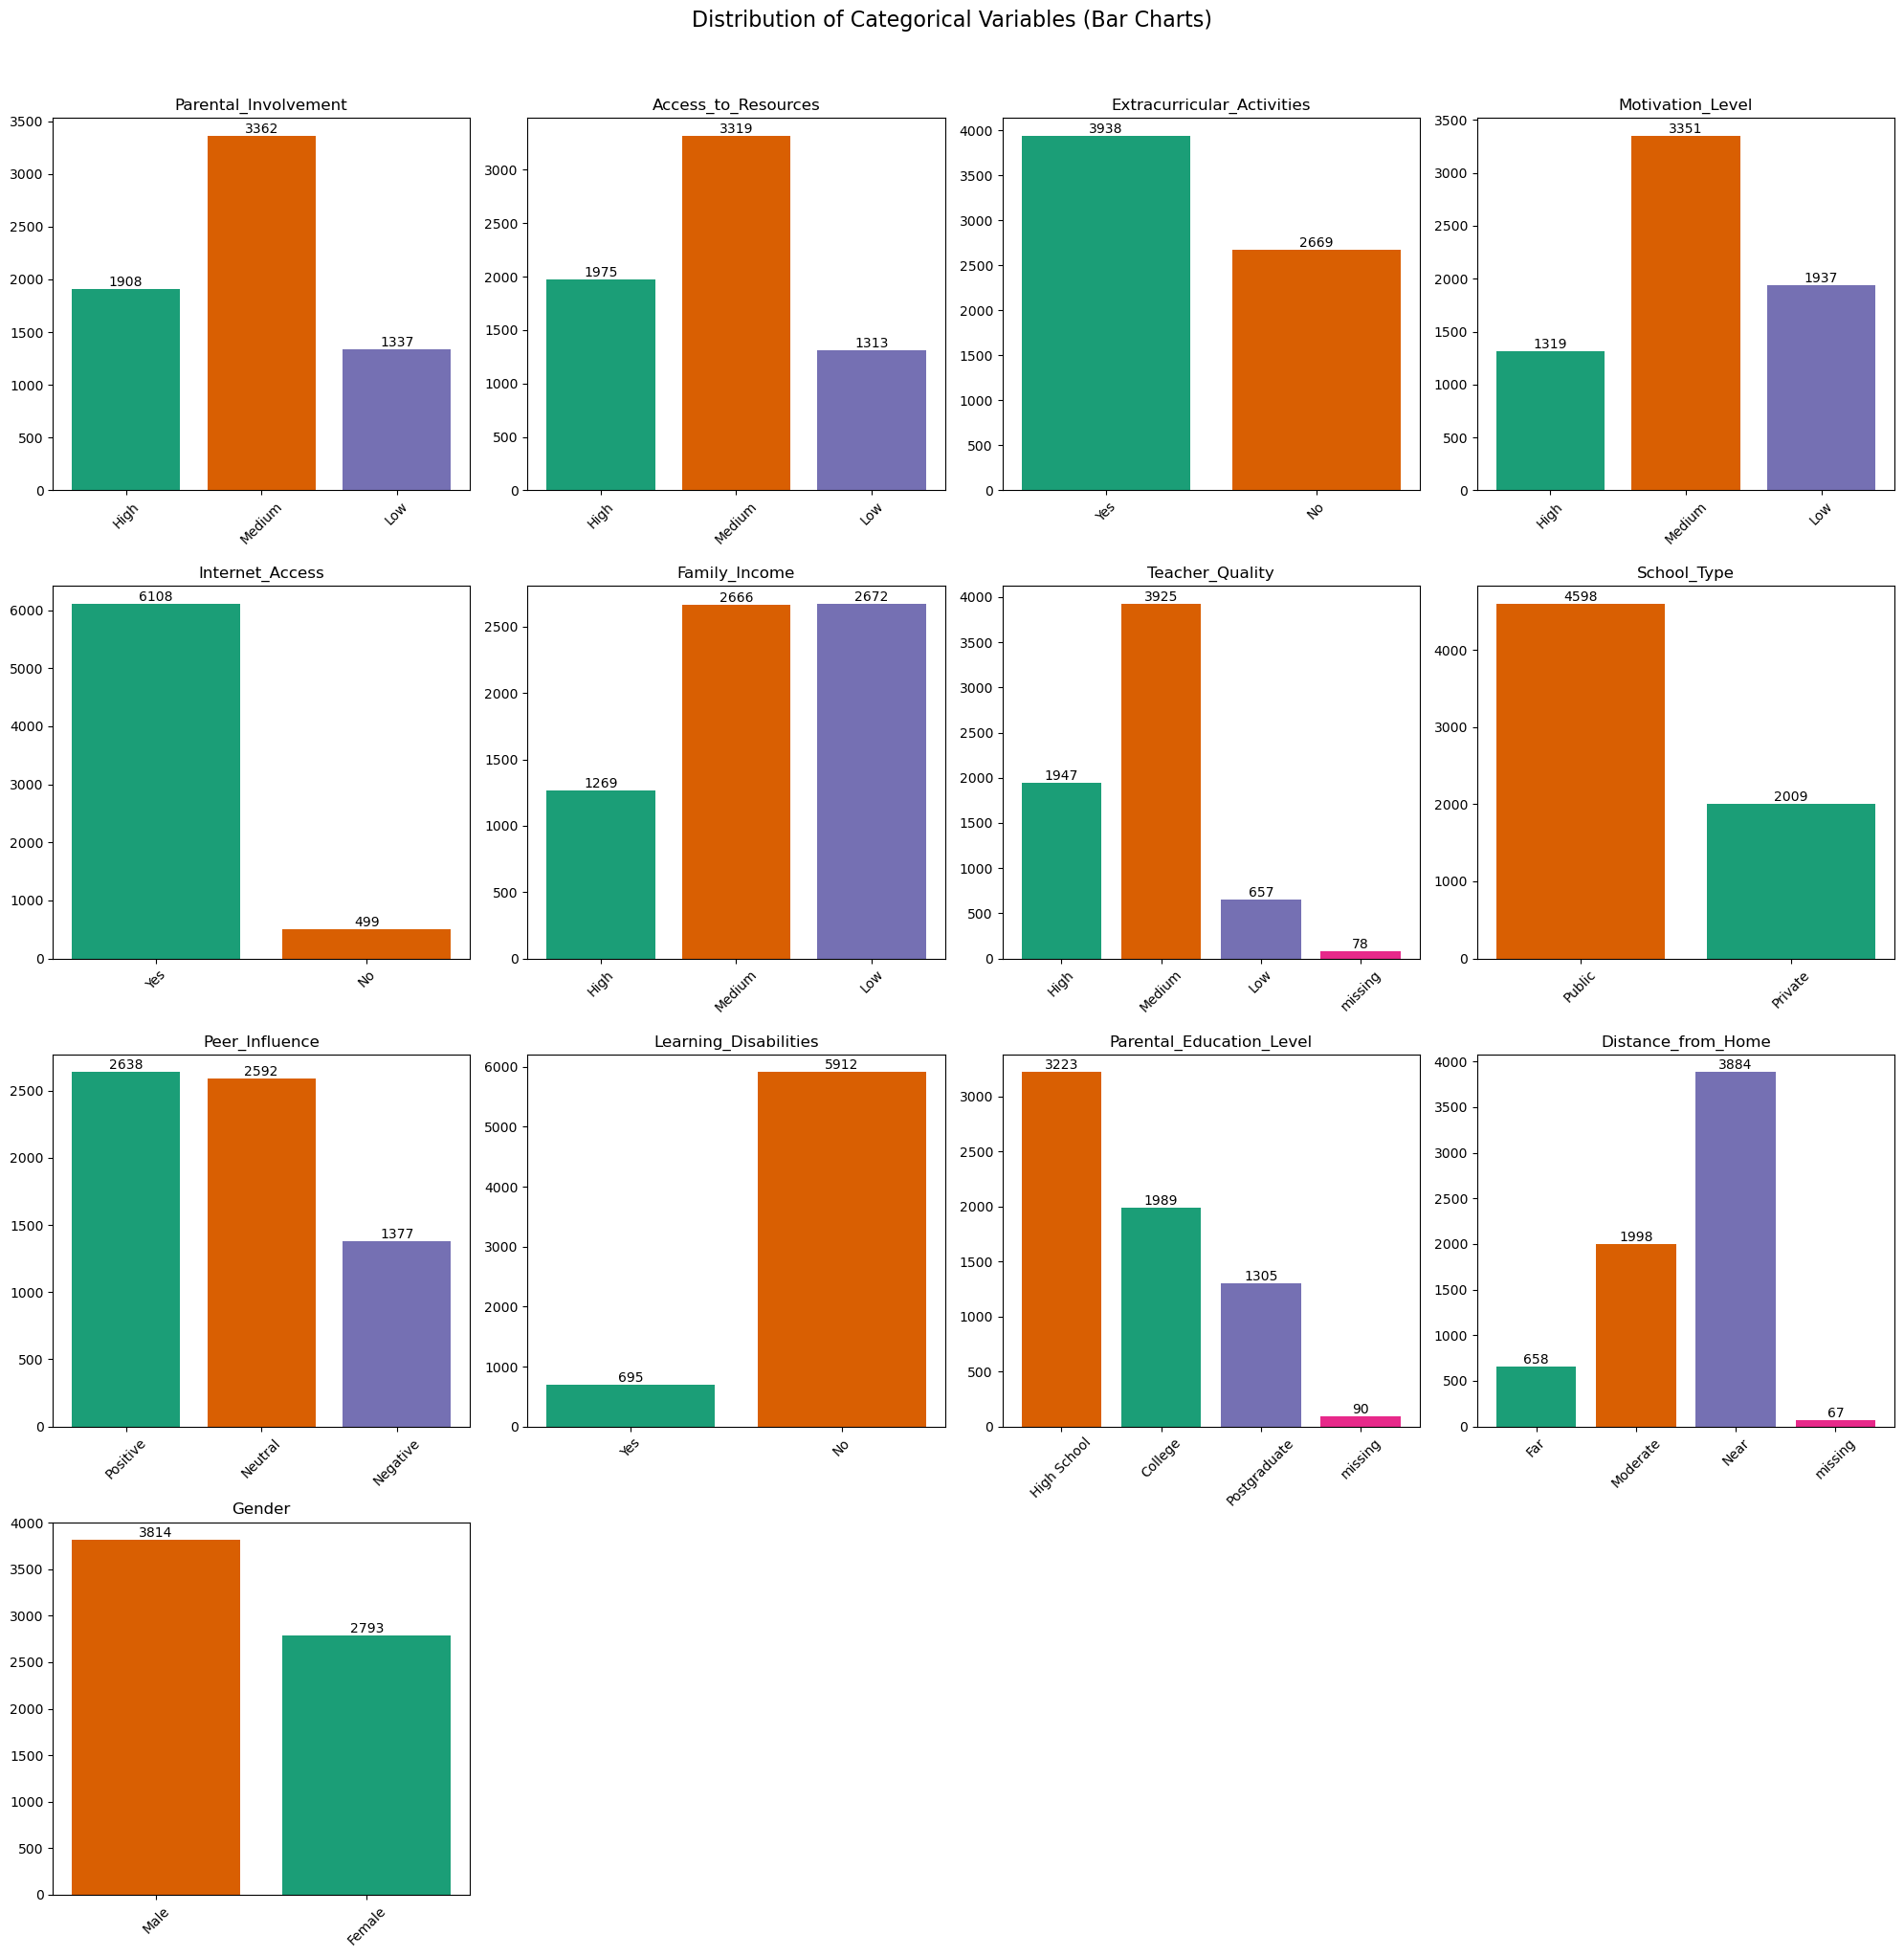
\includegraphics[width=0.9\textwidth]{images/categorical_distribution.png}
    \caption{Distribution of Categorical Variables}
\end{figure}

Key findings from categorical variable analysis:
\begin{itemize}
    \item Most students have medium-level access to resources
    \item Teacher quality is predominantly rated as medium to high
    \item Internet access is available to the majority of students
\end{itemize}

\section{Feature Selection Recommendations}
Based on the EDA, the following feature selection recommendations are made:

\subsection{Key Features to Retain}
\begin{enumerate}
    \item Previous Scores (strong correlation with target variable)
    \item Study Hours (significant predictor)
    \item Teacher Quality (important categorical predictor)
    \item Access to Resources (significant impact on performance)
    \item Internet Access (moderately important factor)
\end{enumerate}

\subsection{Feature Engineering Suggestions}
\begin{itemize}
    \item Create interaction terms between Study Hours and Access to Resources
    \item Consider combining related categorical variables
    \item Transform skewed numerical variables if necessary
\end{itemize}